\section{Model 1: Scratch CNN}
\label{sec:model1}

\subsection{Methods}

The first model is a small Convolutional Neural Network trained from scratch.
It was kept compact on purpose, because the input images are only 64 x 64
pixels and the model is trained without pretrained weights. The architecture
consists of four convolution blocks and one linear classifier.

\begin{table}[H]
\centering
\caption{Architecture of the scratch CNN.}
\label{tab:architecture}
\begin{tabularx}{\textwidth}{lXX}
\toprule
Stage & Layers & Output idea \\
\midrule
Input & RGB image & 3 x 64 x 64 \\
Block 1 & Conv2d 3->32, ReLU, MaxPool & 32 x 32 x 32 \\
Block 2 & Conv2d 32->64, ReLU, MaxPool & 64 x 16 x 16 \\
Block 3 & Conv2d 64->128, ReLU, MaxPool & 128 x 8 x 8 \\
Block 4 & Conv2d 128->256, ReLU, AdaptiveAvgPool & 256 x 1 x 1 \\
Classifier & Flatten, Dropout, Linear & 10 or 2 logits \\
\bottomrule
\end{tabularx}
\end{table}

A CNN was chosen because the images contain local spatial patterns.
Convolutional layers can learn local structures such as vegetation areas,
roads, water surfaces, or dense buildings. ReLU was used as the activation
function because it adds nonlinearity and is simple and stable in deep
networks.

Max pooling reduces the spatial resolution after the first three blocks. This
lowers the computational cost and forces the model to learn more abstract
features. The last block uses adaptive average pooling to 1 x 1, which keeps
the number of parameters before the classifier small.

The model outputs raw logits. No Softmax layer is included in the model during
training. Instead, \texttt{CrossEntropyLoss} is used, which in PyTorch works
directly with logits \cite{pytorch}.

The training loop follows the procedure used in the course: compute
predictions, compute the loss, calculate gradients with backpropagation,
perform the optimizer step, and reset the gradients. The checkpoint with the
lowest validation loss was saved.

The final configuration was selected from the validation experiments in
Section \ref{sec:model1_experiments}. It uses:

\begin{itemize}
  \item \texttt{CrossEntropyLoss},
  \item SGD with momentum 0.9,
  \item learning rate 0.01,
  \item weight decay 1e-4,
  \item dropout 0.3,
  \item batch size 64,
  \item up to 50 epochs.
\end{itemize}

For the 10-class task, the final linear layer has ten outputs. For the binary
task, the same architecture is used with two outputs. This keeps both tasks
directly comparable.

\subsection{Experimental Design}
\label{sec:model1_experiments}

Several experiments were run on the 10-class task to select the final scratch
CNN configuration. The binary task was trained only after this selection. This
keeps the scratch-CNN model selection focused on the harder task.

The ablations E1 to E5 are evaluated only on training and validation data. The
test split was not used for these decisions, because the test split should
remain an independent estimate of the final model performance.

\begin{table}[H]
\centering
\caption{Experiment campaign for the scratch CNN. Test metrics were deliberately
not computed for ablation runs.}
\label{tab:experiments}
\small
\begin{tabularx}{\textwidth}{lXlrrrr}
\toprule
ID & Purpose & Opt. & Epochs & Val Loss & Val Acc. & Val F1 \\
\midrule
E0 & overfit sanity check on 100 images & Adam & 50 & 0.6806 & 0.7400 & 0.7395 \\
E1 & baseline without augmentation & Adam & 29 & 0.1618 & 0.9437 & 0.9419 \\
E2 & augmentation & Adam & 35 & 0.1639 & 0.9472 & 0.9456 \\
E3 & augmentation + dropout/L2 & Adam & 47 & 0.1522 & 0.9504 & 0.9489 \\
E4 & same as E3, but SGD+momentum & SGD & 50 & 0.1362 & 0.9573 & 0.9557 \\
E5 & depthwise-separable convolutions & SGD & 50 & 0.2568 & 0.9121 & 0.9104 \\
\bottomrule
\end{tabularx}
\end{table}

E0 was intended as a sanity check. The model learned the small 100-image subset
clearly better than random guessing, but it did not fully memorize it. The
maximum training accuracy was 0.75. Therefore, E0 should not be interpreted as
a perfect overfitting result, but as evidence that the training loop, model,
and labels are working.

The comparison between E1 and E2 shows a small benefit from augmentation. The
macro-F1 increased from 0.9419 to 0.9456. The validation loss became slightly
worse. For model selection, macro-F1 was more important because it summarizes
performance across all classes and not only the average confidence of the
model.

E3 adds dropout and L2 regularization. This improved the macro-F1 to 0.9489 and
reduced the validation loss to 0.1522. This supports the use of
regularization.

The best validation result was achieved by E4. Compared with E3, only the
optimizer was changed: Adam was replaced by SGD with momentum 0.9. This raised
the macro-F1 to 0.9557 and reduced the validation loss to 0.1362. Therefore,
this configuration was selected for the final runs.

E5 tested whether replacing the standard convolutions with depthwise-separable
convolutions could reduce the model size while keeping similar validation
performance. This variant used 48,424 trainable parameters instead of 390,986.
However, the validation macro-F1 dropped from 0.9557 in E4 to 0.9104 in E5.
The parameter reduction therefore came with a substantial performance cost, so
E5 was not selected for the final test evaluation.

\subsection{Results}

\subsubsection{Final 10-Class Classification}

The final 10-class classification uses the configuration selected in E4. Table
\ref{tab:final_multiclass} shows the validation and test results.

\begin{table}[H]
\centering
\caption{Final results for the 10-class classification task.}
\label{tab:final_multiclass}
\begin{tabular}{lrr}
\toprule
Metric & Validation & Test \\
\midrule
Loss & 0.1362 & 0.1467 \\
Accuracy & 0.9573 & 0.9531 \\
Macro-F1 & 0.9557 & 0.9519 \\
\bottomrule
\end{tabular}
\end{table}

On the test split, 3860 out of 4050 images were classified correctly. This
means that 190 images were misclassified. The validation and test results are
close to each other, which suggests that the selected configuration generalizes
well.

\begin{figure}[H]
\centering
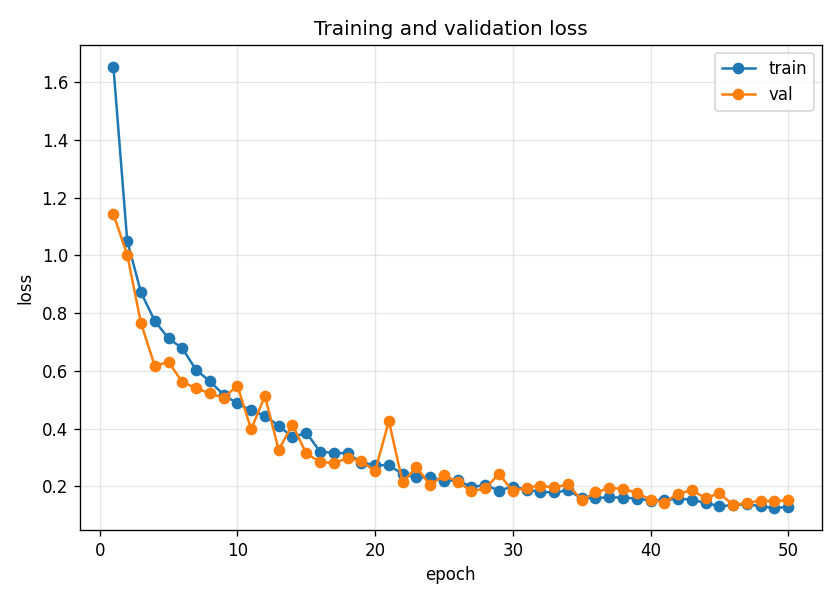
\includegraphics[width=0.78\textwidth]{../outputs/experiments/course_practical/runs/Final_multiclass/plots/loss_curve.png}
\caption{Loss curve of the final 10-class model.}
\label{fig:multiclass_loss}
\end{figure}

\begin{figure}[H]
\centering
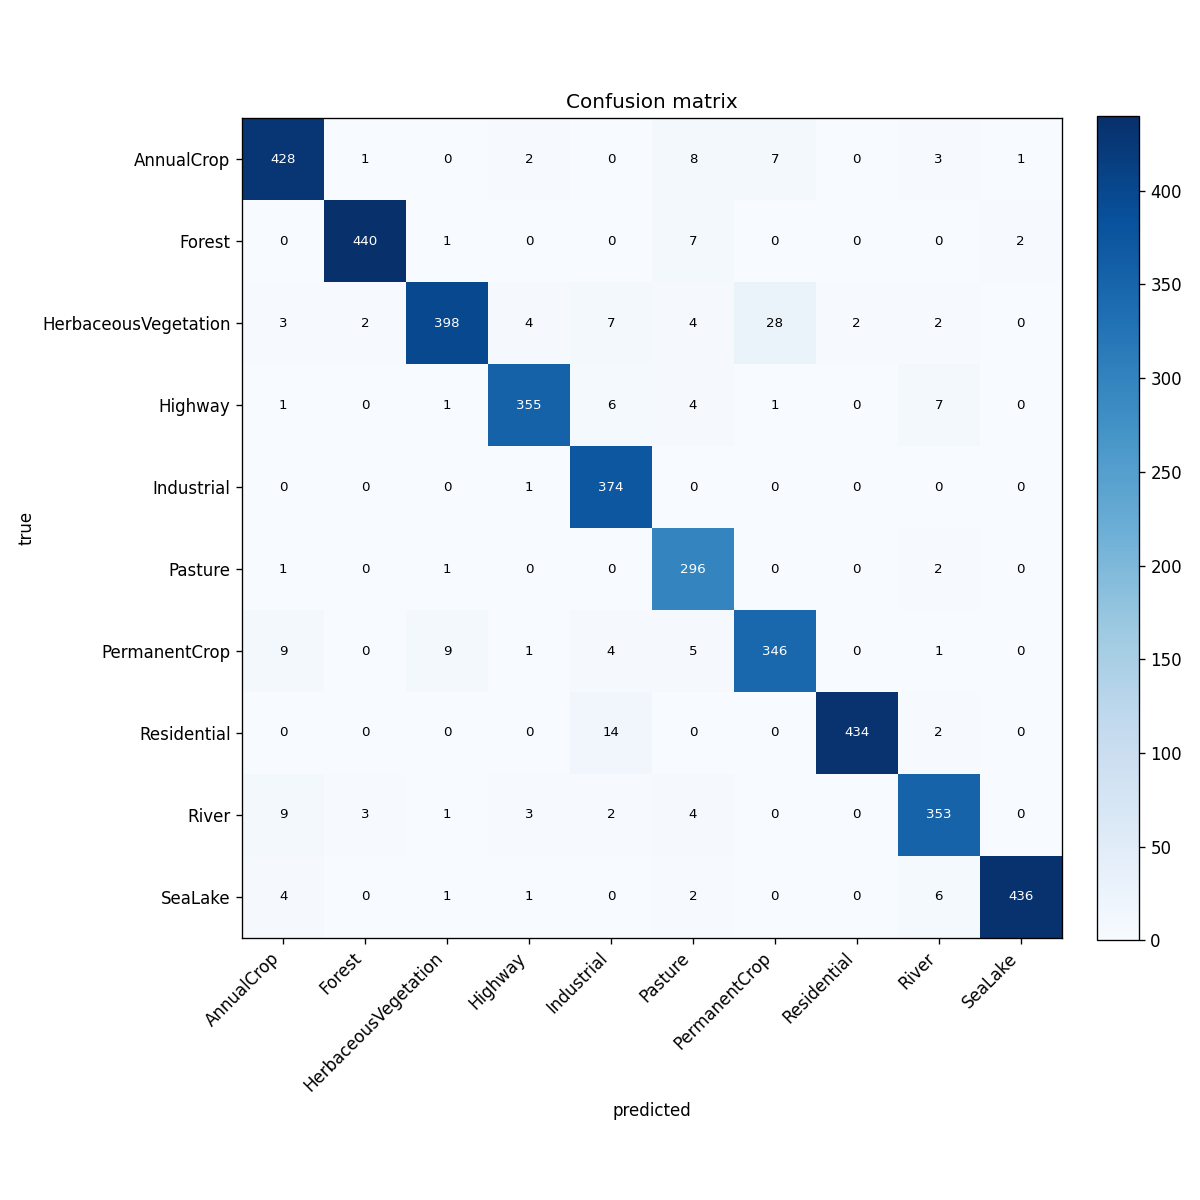
\includegraphics[width=0.78\textwidth]{../outputs/experiments/course_practical/runs/Final_multiclass/plots/confusion_matrix.png}
\caption{Confusion matrix of the final 10-class model on the test split.}
\label{fig:multiclass_cm}
\end{figure}

\begin{table}[H]
\centering
\caption{Per-class test results of the final 10-class model.}
\label{tab:per_class}
\small
\begin{tabular}{lrrrr}
\toprule
Class & Precision & Recall & F1 & Support \\
\midrule
AnnualCrop & 0.9407 & 0.9511 & 0.9459 & 450 \\
Forest & 0.9865 & 0.9778 & 0.9821 & 450 \\
HerbaceousVegetation & 0.9660 & 0.8844 & 0.9234 & 450 \\
Highway & 0.9673 & 0.9467 & 0.9569 & 375 \\
Industrial & 0.9189 & 0.9973 & 0.9565 & 375 \\
Pasture & 0.8970 & 0.9867 & 0.9397 & 300 \\
PermanentCrop & 0.9058 & 0.9227 & 0.9141 & 375 \\
Residential & 0.9954 & 0.9644 & 0.9797 & 450 \\
River & 0.9388 & 0.9413 & 0.9401 & 375 \\
SeaLake & 0.9932 & 0.9689 & 0.9809 & 450 \\
\bottomrule
\end{tabular}
\end{table}

The best F1 scores were achieved for Forest, SeaLake, and Residential. The
weakest scores were obtained for PermanentCrop, HerbaceousVegetation, and
Pasture. This is plausible because these classes can contain visually similar
vegetation patterns. The most frequent confusion in the test split was
HerbaceousVegetation predicted as PermanentCrop, with 28 images.

\subsubsection{Final Binary Classification}

For the binary task, the same selected configuration was used, but with two
output classes. The results are summarized in Table \ref{tab:final_binary}.

\begin{table}[H]
\centering
\caption{Final results for the binary classification task.}
\label{tab:final_binary}
\begin{tabular}{lrr}
\toprule
Metric & Validation & Test \\
\midrule
Loss & 0.0602 & 0.0660 \\
Accuracy & 0.9795 & 0.9795 \\
Macro-F1 & 0.9795 & 0.9795 \\
\bottomrule
\end{tabular}
\end{table}

On the test split, 3967 out of 4050 images were classified correctly. The
binary task is therefore clearly easier than the 10-class task. This is
expected because several similar vegetation classes no longer need to be
separated from each other.

\begin{figure}[H]
\centering
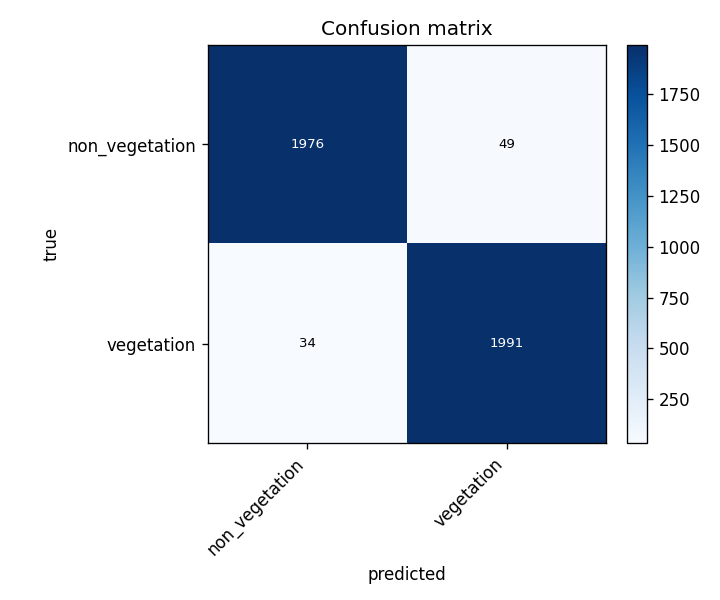
\includegraphics[width=0.7\textwidth]{../outputs/experiments/course_practical/runs/Final_binary/plots/confusion_matrix.png}
\caption{Confusion matrix of the final binary model on the test split.}
\label{fig:binary_cm}
\end{figure}

The binary confusion matrix shows 1976 correctly classified non-vegetation
images and 1991 correctly classified vegetation images. There were 49 cases
where non-vegetation was predicted as vegetation and 34 cases in the opposite
direction.
